\documentclass[1p]{elsarticle_modified}
%\bibliographystyle{elsarticle-num}

%\usepackage[colorlinks]{hyperref}
%\usepackage{abbrmath_seonhwa} %\Abb, \Ascr, \Acal ,\Abf, \Afrak
\usepackage{amsfonts}
\usepackage{amssymb}
\usepackage{amsmath}
\usepackage{amsthm}
\usepackage{scalefnt}
\usepackage{amsbsy}
\usepackage{kotex}
\usepackage{caption}
\usepackage{subfig}
\usepackage{color}
\usepackage{graphicx}
\usepackage{xcolor} %% white, black, red, green, blue, cyan, magenta, yellow
\usepackage{float}
\usepackage{setspace}
\usepackage{hyperref}

\usepackage{tikz}
\usetikzlibrary{arrows}

\usepackage{multirow}
\usepackage{array} % fixed length table
\usepackage{hhline}

%%%%%%%%%%%%%%%%%%%%%
\makeatletter
\renewcommand*\env@matrix[1][\arraystretch]{%
	\edef\arraystretch{#1}%
	\hskip -\arraycolsep
	\let\@ifnextchar\new@ifnextchar
	\array{*\c@MaxMatrixCols c}}
\makeatother %https://tex.stackexchange.com/questions/14071/how-can-i-increase-the-line-spacing-in-a-matrix
%%%%%%%%%%%%%%%

\usepackage[normalem]{ulem}

\newcommand{\msout}[1]{\ifmmode\text{\sout{\ensuremath{#1}}}\else\sout{#1}\fi}
%SOURCE: \msout is \stkout macro in https://tex.stackexchange.com/questions/20609/strikeout-in-math-mode

\newcommand{\cancel}[1]{
	\ifmmode
	{\color{red}\msout{#1}}
	\else
	{\color{red}\sout{#1}}
	\fi
}

\newcommand{\add}[1]{
	{\color{blue}\uwave{#1}}
}

\newcommand{\replace}[2]{
	\ifmmode
	{\color{red}\msout{#1}}{\color{blue}\uwave{#2}}
	\else
	{\color{red}\sout{#1}}{\color{blue}\uwave{#2}}
	\fi
}

\newcommand{\Sol}{\mathcal{S}} %segment
\newcommand{\D}{D} %diagram
\newcommand{\A}{\mathcal{A}} %arc


%%%%%%%%%%%%%%%%%%%%%%%%%%%%%5 test

\def\sl{\operatorname{\textup{SL}}(2,\Cbb)}
\def\psl{\operatorname{\textup{PSL}}(2,\Cbb)}
\def\quan{\mkern 1mu \triangleright \mkern 1mu}

\theoremstyle{definition}
\newtheorem{thm}{Theorem}[section]
\newtheorem{prop}[thm]{Proposition}
\newtheorem{lem}[thm]{Lemma}
\newtheorem{ques}[thm]{Question}
\newtheorem{cor}[thm]{Corollary}
\newtheorem{defn}[thm]{Definition}
\newtheorem{exam}[thm]{Example}
\newtheorem{rmk}[thm]{Remark}
\newtheorem{alg}[thm]{Algorithm}

\newcommand{\I}{\sqrt{-1}}
\begin{document}

%\begin{frontmatter}
%
%\title{Boundary parabolic representations of knots up to 8 crossings}
%
%%% Group authors per affiliation:
%\author{Yunhi Cho} 
%\address{Department of Mathematics, University of Seoul, Seoul, Korea}
%\ead{yhcho@uos.ac.kr}
%
%
%\author{Seonhwa Kim} %\fnref{s_kim}}
%\address{Center for Geometry and Physics, Institute for Basic Science, Pohang, 37673, Korea}
%\ead{ryeona17@ibs.re.kr}
%
%\author{Hyuk Kim}
%\address{Department of Mathematical Sciences, Seoul National University, Seoul 08826, Korea}
%\ead{hyukkim@snu.ac.kr}
%
%\author{Seokbeom Yoon}
%\address{Department of Mathematical Sciences, Seoul National University, Seoul, 08826,  Korea}
%\ead{sbyoon15@snu.ac.kr}
%
%\begin{abstract}
%We find all boundary parabolic representation of knots up to 8 crossings.
%
%\end{abstract}
%\begin{keyword}
%    \MSC[2010] 57M25 
%\end{keyword}
%
%\end{frontmatter}

%\linenumbers
%\tableofcontents
%
\newcommand\colored[1]{\textcolor{white}{\rule[-0.35ex]{0.8em}{1.4ex}}\kern-0.8em\color{red} #1}%
%\newcommand\colored[1]{\textcolor{white}{ #1}\kern-2.17ex	\textcolor{white}{ #1}\kern-1.81ex	\textcolor{white}{ #1}\kern-2.15ex\color{red}#1	}

{\Large $\underline{12n_{0835}~(K12n_{0835})}$}

\setlength{\tabcolsep}{10pt}
\renewcommand{\arraystretch}{1.6}
\vspace{1cm}\begin{tabular}{m{100pt}>{\centering\arraybackslash}m{274pt}}
\multirow{5}{120pt}{
	\centering
	\includegraphics[width=112pt]{../../../GIT/diagram.site/Diagrams/png/2924_12n_0835.png}\\
\ \ \ A knot diagram\footnotemark}&
\allowdisplaybreaks
\textbf{Linearized knot diagam} \\
\cline{2-2}
 &
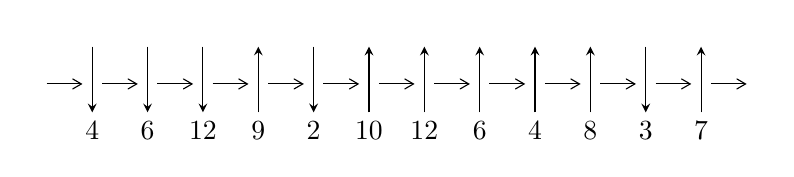
\begin{tikzpicture}[x=20pt, y=17pt]
	% nodes
	\node (C0) at (0, 0) {};
	\node (C1) at (1, 0) {};
	\node (C1U) at (1, +1) {};
	\node (C1D) at (1, -1) {4};

	\node (C2) at (2, 0) {};
	\node (C2U) at (2, +1) {};
	\node (C2D) at (2, -1) {6};

	\node (C3) at (3, 0) {};
	\node (C3U) at (3, +1) {};
	\node (C3D) at (3, -1) {12};

	\node (C4) at (4, 0) {};
	\node (C4U) at (4, +1) {};
	\node (C4D) at (4, -1) {9};

	\node (C5) at (5, 0) {};
	\node (C5U) at (5, +1) {};
	\node (C5D) at (5, -1) {2};

	\node (C6) at (6, 0) {};
	\node (C6U) at (6, +1) {};
	\node (C6D) at (6, -1) {10};

	\node (C7) at (7, 0) {};
	\node (C7U) at (7, +1) {};
	\node (C7D) at (7, -1) {12};

	\node (C8) at (8, 0) {};
	\node (C8U) at (8, +1) {};
	\node (C8D) at (8, -1) {6};

	\node (C9) at (9, 0) {};
	\node (C9U) at (9, +1) {};
	\node (C9D) at (9, -1) {4};

	\node (C10) at (10, 0) {};
	\node (C10U) at (10, +1) {};
	\node (C10D) at (10, -1) {8};

	\node (C11) at (11, 0) {};
	\node (C11U) at (11, +1) {};
	\node (C11D) at (11, -1) {3};

	\node (C12) at (12, 0) {};
	\node (C12U) at (12, +1) {};
	\node (C12D) at (12, -1) {7};
	\node (C13) at (13, 0) {};

	% arrows
	\draw[->,>={angle 60}]
	(C0) edge (C1) (C1) edge (C2) (C2) edge (C3) (C3) edge (C4) (C4) edge (C5) (C5) edge (C6) (C6) edge (C7) (C7) edge (C8) (C8) edge (C9) (C9) edge (C10) (C10) edge (C11) (C11) edge (C12) (C12) edge (C13) ;	\draw[->,>=stealth]
	(C1U) edge (C1D) (C2U) edge (C2D) (C3U) edge (C3D) (C4D) edge (C4U) (C5U) edge (C5D) (C6D) edge (C6U) (C7D) edge (C7U) (C8D) edge (C8U) (C9D) edge (C9U) (C10D) edge (C10U) (C11U) edge (C11D) (C12D) edge (C12U) ;
	\end{tikzpicture} \\
\hhline{~~} \\& 
\textbf{Solving Sequence} \\ \cline{2-2} 
 &
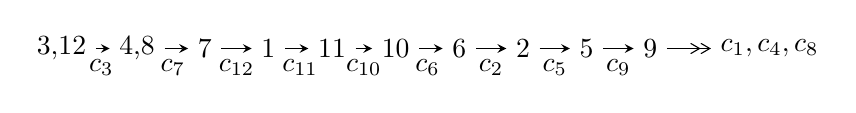
\begin{tikzpicture}[x=23pt, y=7pt]
	% node
	\node (A0) at (-1/8, 0) {3,12};
	\node (A1) at (17/16, 0) {4,8};
	\node (A2) at (17/8, 0) {7};
	\node (A3) at (25/8, 0) {1};
	\node (A4) at (33/8, 0) {11};
	\node (A5) at (41/8, 0) {10};
	\node (A6) at (49/8, 0) {6};
	\node (A7) at (57/8, 0) {2};
	\node (A8) at (65/8, 0) {5};
	\node (A9) at (73/8, 0) {9};
	\node (C1) at (1/2, -1) {$c_{3}$};
	\node (C2) at (13/8, -1) {$c_{7}$};
	\node (C3) at (21/8, -1) {$c_{12}$};
	\node (C4) at (29/8, -1) {$c_{11}$};
	\node (C5) at (37/8, -1) {$c_{10}$};
	\node (C6) at (45/8, -1) {$c_{6}$};
	\node (C7) at (53/8, -1) {$c_{2}$};
	\node (C8) at (61/8, -1) {$c_{5}$};
	\node (C9) at (69/8, -1) {$c_{9}$};
	\node (A10) at (11, 0) {$c_{1},c_{4},c_{8}$};

	% edge
	\draw[->,>=stealth]	
	(A0) edge (A1) (A1) edge (A2) (A2) edge (A3) (A3) edge (A4) (A4) edge (A5) (A5) edge (A6) (A6) edge (A7) (A7) edge (A8) (A8) edge (A9) ;
	\draw[->>,>={angle 60}]	
	(A9) edge (A10);
\end{tikzpicture} \\ 

\end{tabular} \\

\footnotetext{
The image of knot diagram is generated by the software ``\textbf{Draw programme}" developed by Andrew Bartholomew(\url{http://www.layer8.co.uk/maths/draw/index.htm\#Running-draw}), where we modified some parts for our purpose(\url{https://github.com/CATsTAILs/LinksPainter}).
}\phantom \\ \newline 
\centering \textbf{Ideals for irreducible components\footnotemark of $X_{\text{par}}$} 
 
\begin{align*}
I^u_{1}&=\langle 
-11962 u^{12}-32982 u^{11}+\cdots+180027 b-81583,\\
\phantom{I^u_{1}}&\phantom{= \langle  }-51167 u^{12}-51141 u^{11}+\cdots+180027 a+431806,\\
\phantom{I^u_{1}}&\phantom{= \langle  }u^{13}+2 u^{12}+u^{11}-12 u^{10}-10 u^9+12 u^8+39 u^7+u^6-48 u^5-18 u^4+21 u^3+18 u^2+3 u-1\rangle \\
I^u_{2}&=\langle 
b,\;a+u,\;u^3- u^2+1\rangle \\
I^u_{3}&=\langle 
34532 u^{11}-8910 u^{10}+\cdots+191471 b-108223,\\
\phantom{I^u_{3}}&\phantom{= \langle  }126317 u^{11}-132222 u^{10}+\cdots+191471 a-196501,\\
\phantom{I^u_{3}}&\phantom{= \langle  }u^{12}-2 u^{11}+u^{10}-16 u^8+14 u^7+29 u^6-12 u^5+4 u^4+16 u^3-5 u^2-2 u+1\rangle \\
I^u_{4}&=\langle 
-188 u^7-516 u^6-1817 u^5-4442 u^4-8033 u^3-9745 u^2+4095 b-9869 u-4774,\\
\phantom{I^u_{4}}&\phantom{= \langle  }209 u^7+138 u^6+2216 u^5+5156 u^4+6164 u^3+20875 u^2+28665 a+9512 u+2737,\\
\phantom{I^u_{4}}&\phantom{= \langle  }u^8+2 u^7+10 u^6+24 u^5+45 u^4+76 u^3+92 u^2+70 u+49\rangle \\
\\
\end{align*}
\raggedright * 4 irreducible components of $\dim_{\mathbb{C}}=0$, with total 36 representations.\\
\footnotetext{All coefficients of polynomials are rational numbers. But the coefficients are sometimes approximated in decimal forms when there is not enough margin.}
\newpage
\renewcommand{\arraystretch}{1}
\centering \section*{I. $I^u_{1}= \langle -1.20\times10^{4} u^{12}-3.30\times10^{4} u^{11}+\cdots+1.80\times10^{5} b-8.16\times10^{4},\;-5.12\times10^{4} u^{12}-5.11\times10^{4} u^{11}+\cdots+1.80\times10^{5} a+4.32\times10^{5},\;u^{13}+2 u^{12}+\cdots+3 u-1 \rangle$}
\flushleft \textbf{(i) Arc colorings}\\
\begin{tabular}{m{7pt} m{180pt} m{7pt} m{180pt} }
\flushright $a_{3}=$&$\begin{pmatrix}1\\0\end{pmatrix}$ \\
\flushright $a_{12}=$&$\begin{pmatrix}0\\u\end{pmatrix}$ \\
\flushright $a_{4}=$&$\begin{pmatrix}1\\u^2\end{pmatrix}$ \\
\flushright $a_{8}=$&$\begin{pmatrix}0.284218 u^{12}+0.284074 u^{11}+\cdots-3.97384 u-2.39856\\0.0664456 u^{12}+0.183206 u^{11}+\cdots+0.314458 u+0.453171\end{pmatrix}$ \\
\flushright $a_{7}=$&$\begin{pmatrix}0.284218 u^{12}+0.284074 u^{11}+\cdots-3.97384 u-2.39856\\0.0888700 u^{12}+0.283657 u^{11}+\cdots+1.45177 u+0.168808\end{pmatrix}$ \\
\flushright $a_{1}=$&$\begin{pmatrix}0.0237131 u^{12}-0.0981353 u^{11}+\cdots-2.62369 u+1.88978\\0.105179 u^{12}+0.356713 u^{11}+\cdots-0.902920 u+0.234726\end{pmatrix}$ \\
\flushright $a_{11}=$&$\begin{pmatrix}u\\u\end{pmatrix}$ \\
\flushright $a_{10}=$&$\begin{pmatrix}-0.222456 u^{12}-0.0646236 u^{11}+\cdots+1.26037 u-1.50950\\0.0856205 u^{12}+0.383542 u^{11}+\cdots+1.88790 u+0.0960689\end{pmatrix}$ \\
\flushright $a_{6}=$&$\begin{pmatrix}-0.509496 u^{12}-1.24145 u^{11}+\cdots-8.54774 u-0.268115\\u\end{pmatrix}$ \\
\flushright $a_{2}=$&$\begin{pmatrix}0.222456 u^{12}+0.0646236 u^{11}+\cdots-1.26037 u+1.50950\\- u^2\end{pmatrix}$ \\
\flushright $a_{5}=$&$\begin{pmatrix}-0.889783 u^{12}-1.80328 u^{11}+\cdots-7.70561 u-0.0456598\\- u^3+u\end{pmatrix}$ \\
\flushright $a_{9}=$&$\begin{pmatrix}-0.506818 u^{12}-0.610925 u^{11}+\cdots-1.99085 u-1.22528\\0.141223 u^{12}+0.341066 u^{11}+\cdots+1.53626 u+0.118493\end{pmatrix}$\\&\end{tabular}
\flushleft \textbf{(ii) Obstruction class $= -1$}\\~\\
\flushleft \textbf{(iii) Cusp Shapes $= \frac{133277}{60009} u^{12}+\frac{97412}{20003} u^{11}+\cdots+\frac{2500157}{60009} u+\frac{279872}{60009}$}\\~\\
\newpage\renewcommand{\arraystretch}{1}
\flushleft \textbf{(iv) u-Polynomials at the component}\newline \\
\begin{tabular}{m{50pt}|m{274pt}}
Crossings & \hspace{64pt}u-Polynomials at each crossing \\
\hline $$\begin{aligned}c_{1}\end{aligned}$$&$\begin{aligned}
&u^{13}+2 u^{12}+\cdots+73 u+5
\end{aligned}$\\
\hline $$\begin{aligned}c_{2},c_{3},c_{5}\\c_{11}\end{aligned}$$&$\begin{aligned}
&u^{13}+2 u^{12}+\cdots+3 u-1
\end{aligned}$\\
\hline $$\begin{aligned}c_{4},c_{7},c_{9}\\c_{12}\end{aligned}$$&$\begin{aligned}
&u^{13}+10 u^{11}+\cdots-12 u-4
\end{aligned}$\\
\hline $$\begin{aligned}c_{6}\end{aligned}$$&$\begin{aligned}
&u^{13}-3 u^{12}+\cdots+112 u-19
\end{aligned}$\\
\hline $$\begin{aligned}c_{8},c_{10}\end{aligned}$$&$\begin{aligned}
&u^{13}+2 u^{12}+\cdots+5 u-1
\end{aligned}$\\
\hline
\end{tabular}\\~\\
\newpage\renewcommand{\arraystretch}{1}
\flushleft \textbf{(v) Riley Polynomials at the component}\newline \\
\begin{tabular}{m{50pt}|m{274pt}}
Crossings & \hspace{64pt}Riley Polynomials at each crossing \\
\hline $$\begin{aligned}c_{1}\end{aligned}$$&$\begin{aligned}
&y^{13}-38 y^{12}+\cdots+7329 y-25
\end{aligned}$\\
\hline $$\begin{aligned}c_{2},c_{3},c_{5}\\c_{11}\end{aligned}$$&$\begin{aligned}
&y^{13}-2 y^{12}+\cdots+45 y-1
\end{aligned}$\\
\hline $$\begin{aligned}c_{4},c_{7},c_{9}\\c_{12}\end{aligned}$$&$\begin{aligned}
&y^{13}+20 y^{12}+\cdots+208 y-16
\end{aligned}$\\
\hline $$\begin{aligned}c_{6}\end{aligned}$$&$\begin{aligned}
&y^{13}+7 y^{12}+\cdots+2094 y-361
\end{aligned}$\\
\hline $$\begin{aligned}c_{8},c_{10}\end{aligned}$$&$\begin{aligned}
&y^{13}-8 y^{12}+\cdots+7 y-1
\end{aligned}$\\
\hline
\end{tabular}\\~\\
\newpage\flushleft \textbf{(vi) Complex Volumes and Cusp Shapes}
$$\begin{array}{c|c|c}  
\text{Solutions to }I^u_{1}& \I (\text{vol} + \sqrt{-1}CS) & \text{Cusp shape}\\
 \hline 
\begin{aligned}
u &= \phantom{-}1.122400 + 0.448785 I \\
a &= \phantom{-}0.292793 + 0.874754 I \\
b &= -0.109259 + 0.767460 I\end{aligned}
 & -6.52437 - 4.35431 I & -2.69323 + 5.57961 I \\ \hline\begin{aligned}
u &= \phantom{-}1.122400 - 0.448785 I \\
a &= \phantom{-}0.292793 - 0.874754 I \\
b &= -0.109259 - 0.767460 I\end{aligned}
 & -6.52437 + 4.35431 I & -2.69323 - 5.57961 I \\ \hline\begin{aligned}
u &= -0.749285 + 0.043693 I \\
a &= -0.509626 + 0.065149 I \\
b &= -0.738849 + 0.256795 I\end{aligned}
 & -1.302700 + 0.032683 I & -7.31648 - 0.16173 I \\ \hline\begin{aligned}
u &= -0.749285 - 0.043693 I \\
a &= -0.509626 - 0.065149 I \\
b &= -0.738849 - 0.256795 I\end{aligned}
 & -1.302700 - 0.032683 I & -7.31648 + 0.16173 I \\ \hline\begin{aligned}
u &= \phantom{-}1.265880 + 0.291483 I \\
a &= \phantom{-}0.18470 - 1.44719 I \\
b &= -0.35048 - 2.57213 I\end{aligned}
 & -14.5051 - 3.1980 I & -6.84015 + 2.15870 I \\ \hline\begin{aligned}
u &= \phantom{-}1.265880 - 0.291483 I \\
a &= \phantom{-}0.18470 + 1.44719 I \\
b &= -0.35048 + 2.57213 I\end{aligned}
 & -14.5051 + 3.1980 I & -6.84015 - 2.15870 I \\ \hline\begin{aligned}
u &= -0.438416 + 0.418996 I \\
a &= \phantom{-}1.83391 - 1.67711 I \\
b &= \phantom{-}0.675501 + 0.073236 I\end{aligned}
 & -8.52319 + 2.72289 I & -7.74001 - 0.35750 I \\ \hline\begin{aligned}
u &= -0.438416 - 0.418996 I \\
a &= \phantom{-}1.83391 + 1.67711 I \\
b &= \phantom{-}0.675501 - 0.073236 I\end{aligned}
 & -8.52319 - 2.72289 I & -7.74001 + 0.35750 I \\ \hline\begin{aligned}
u &= -0.86722 + 1.24197 I \\
a &= \phantom{-}0.518889 - 0.563420 I \\
b &= \phantom{-}0.04501 - 1.85139 I\end{aligned}
 & \phantom{-}4.79571 + 2.82647 I & -1.37286 - 2.37043 I \\ \hline\begin{aligned}
u &= -0.86722 - 1.24197 I \\
a &= \phantom{-}0.518889 + 0.563420 I \\
b &= \phantom{-}0.04501 + 1.85139 I\end{aligned}
 & \phantom{-}4.79571 - 2.82647 I & -1.37286 + 2.37043 I\\
 \hline 
 \end{array}$$\newpage$$\begin{array}{c|c|c}  
\text{Solutions to }I^u_{1}& \I (\text{vol} + \sqrt{-1}CS) & \text{Cusp shape}\\
 \hline 
\begin{aligned}
u &= \phantom{-}0.158979\phantom{ +0.000000I} \\
a &= -2.81443\phantom{ +0.000000I} \\
b &= \phantom{-}0.486240\phantom{ +0.000000I}\end{aligned}
 & \phantom{-}0.852515\phantom{ +0.000000I} & \phantom{-}11.9090\phantom{ +0.000000I} \\ \hline\begin{aligned}
u &= -1.41284 + 1.83586 I \\
a &= -0.413448 + 0.805929 I \\
b &= -0.26505 + 2.03068 I\end{aligned}
 & \phantom{-}0.95941 + 10.95210 I & -1.49177 - 4.40872 I \\ \hline\begin{aligned}
u &= -1.41284 - 1.83586 I \\
a &= -0.413448 - 0.805929 I \\
b &= -0.26505 - 2.03068 I\end{aligned}
 & \phantom{-}0.95941 - 10.95210 I & -1.49177 + 4.40872 I\\
 \hline 
 \end{array}$$\newpage\newpage\renewcommand{\arraystretch}{1}
\centering \section*{II. $I^u_{2}= \langle b,\;a+u,\;u^3- u^2+1 \rangle$}
\flushleft \textbf{(i) Arc colorings}\\
\begin{tabular}{m{7pt} m{180pt} m{7pt} m{180pt} }
\flushright $a_{3}=$&$\begin{pmatrix}1\\0\end{pmatrix}$ \\
\flushright $a_{12}=$&$\begin{pmatrix}0\\u\end{pmatrix}$ \\
\flushright $a_{4}=$&$\begin{pmatrix}1\\u^2\end{pmatrix}$ \\
\flushright $a_{8}=$&$\begin{pmatrix}- u\\0\end{pmatrix}$ \\
\flushright $a_{7}=$&$\begin{pmatrix}- u\\- u^2+1\end{pmatrix}$ \\
\flushright $a_{1}=$&$\begin{pmatrix}u^2-1\\-1\end{pmatrix}$ \\
\flushright $a_{11}=$&$\begin{pmatrix}u\\u\end{pmatrix}$ \\
\flushright $a_{10}=$&$\begin{pmatrix}- u^2+u+1\\u\end{pmatrix}$ \\
\flushright $a_{6}=$&$\begin{pmatrix}2 u^2- u-1\\- u\end{pmatrix}$ \\
\flushright $a_{2}=$&$\begin{pmatrix}u^2- u-1\\- u^2\end{pmatrix}$ \\
\flushright $a_{5}=$&$\begin{pmatrix}2 u^2\\u^2- u-1\end{pmatrix}$ \\
\flushright $a_{9}=$&$\begin{pmatrix}u+1\\u^2-1\end{pmatrix}$\\&\end{tabular}
\flushleft \textbf{(ii) Obstruction class $= 1$}\\~\\
\flushleft \textbf{(iii) Cusp Shapes $= 6 u^2-4 u-3$}\\~\\
\newpage\renewcommand{\arraystretch}{1}
\flushleft \textbf{(iv) u-Polynomials at the component}\newline \\
\begin{tabular}{m{50pt}|m{274pt}}
Crossings & \hspace{64pt}u-Polynomials at each crossing \\
\hline $$\begin{aligned}c_{1},c_{2},c_{11}\end{aligned}$$&$\begin{aligned}
&u^3+u^2-1
\end{aligned}$\\
\hline $$\begin{aligned}c_{3},c_{5}\end{aligned}$$&$\begin{aligned}
&u^3- u^2+1
\end{aligned}$\\
\hline $$\begin{aligned}c_{4},c_{7}\end{aligned}$$&$\begin{aligned}
&u^3+u^2+2 u+1
\end{aligned}$\\
\hline $$\begin{aligned}c_{6}\end{aligned}$$&$\begin{aligned}
&u^3+2 u^2+3 u+1
\end{aligned}$\\
\hline $$\begin{aligned}c_{8},c_{9},c_{10}\\c_{12}\end{aligned}$$&$\begin{aligned}
&u^3- u^2+2 u-1
\end{aligned}$\\
\hline
\end{tabular}\\~\\
\newpage\renewcommand{\arraystretch}{1}
\flushleft \textbf{(v) Riley Polynomials at the component}\newline \\
\begin{tabular}{m{50pt}|m{274pt}}
Crossings & \hspace{64pt}Riley Polynomials at each crossing \\
\hline $$\begin{aligned}c_{1},c_{2},c_{3}\\c_{5},c_{11}\end{aligned}$$&$\begin{aligned}
&y^3- y^2+2 y-1
\end{aligned}$\\
\hline $$\begin{aligned}c_{4},c_{7},c_{8}\\c_{9},c_{10},c_{12}\end{aligned}$$&$\begin{aligned}
&y^3+3 y^2+2 y-1
\end{aligned}$\\
\hline $$\begin{aligned}c_{6}\end{aligned}$$&$\begin{aligned}
&y^3+2 y^2+5 y-1
\end{aligned}$\\
\hline
\end{tabular}\\~\\
\newpage\flushleft \textbf{(vi) Complex Volumes and Cusp Shapes}
$$\begin{array}{c|c|c}  
\text{Solutions to }I^u_{2}& \I (\text{vol} + \sqrt{-1}CS) & \text{Cusp shape}\\
 \hline 
\begin{aligned}
u &= \phantom{-}0.877439 + 0.744862 I \\
a &= -0.877439 - 0.744862 I \\
b &= \phantom{-0.000000 } 0\end{aligned}
 & -8.03068 - 3.77083 I & -5.21928 + 4.86340 I \\ \hline\begin{aligned}
u &= \phantom{-}0.877439 - 0.744862 I \\
a &= -0.877439 + 0.744862 I \\
b &= \phantom{-0.000000 } 0\end{aligned}
 & -8.03068 + 3.77083 I & -5.21928 - 4.86340 I \\ \hline\begin{aligned}
u &= -0.754878\phantom{ +0.000000I} \\
a &= \phantom{-}0.754878\phantom{ +0.000000I} \\
b &= \phantom{-0.000000 } 0\end{aligned}
 & -0.387983\phantom{ +0.000000I} & \phantom{-}3.43860\phantom{ +0.000000I}\\
 \hline 
 \end{array}$$\newpage\newpage\renewcommand{\arraystretch}{1}
\centering \section*{III. $I^u_{3}= \langle 34532 u^{11}-8910 u^{10}+\cdots+191471 b-108223,\;1.26\times10^{5} u^{11}-1.32\times10^{5} u^{10}+\cdots+1.91\times10^{5} a-1.97\times10^{5},\;u^{12}-2 u^{11}+\cdots-2 u+1 \rangle$}
\flushleft \textbf{(i) Arc colorings}\\
\begin{tabular}{m{7pt} m{180pt} m{7pt} m{180pt} }
\flushright $a_{3}=$&$\begin{pmatrix}1\\0\end{pmatrix}$ \\
\flushright $a_{12}=$&$\begin{pmatrix}0\\u\end{pmatrix}$ \\
\flushright $a_{4}=$&$\begin{pmatrix}1\\u^2\end{pmatrix}$ \\
\flushright $a_{8}=$&$\begin{pmatrix}-0.659719 u^{11}+0.690559 u^{10}+\cdots-6.35697 u+1.02627\\-0.180351 u^{11}+0.0465345 u^{10}+\cdots-1.55862 u+0.565219\end{pmatrix}$ \\
\flushright $a_{7}=$&$\begin{pmatrix}-0.659719 u^{11}+0.690559 u^{10}+\cdots-6.35697 u+1.02627\\-0.460054 u^{11}+0.535402 u^{10}+\cdots-2.15666 u+1.19410\end{pmatrix}$ \\
\flushright $a_{1}=$&$\begin{pmatrix}1.65524 u^{11}-2.78398 u^{10}+\cdots-1.00772 u-6.09660\\0.224859 u^{11}-0.296390 u^{10}+\cdots-0.503115 u-1.64700\end{pmatrix}$ \\
\flushright $a_{11}=$&$\begin{pmatrix}u\\u\end{pmatrix}$ \\
\flushright $a_{10}=$&$\begin{pmatrix}-1.52166 u^{11}+2.61616 u^{10}+\cdots+1.10685 u+4.97611\\-0.129111 u^{11}+0.261251 u^{10}+\cdots+1.26558 u+1.19082\end{pmatrix}$ \\
\flushright $a_{6}=$&$\begin{pmatrix}-1.16060 u^{11}+2.08065 u^{10}+\cdots+1.32344 u+4.67364\\-0.250257 u^{11}+0.475545 u^{10}+\cdots-0.181777 u+1.44895\end{pmatrix}$ \\
\flushright $a_{2}=$&$\begin{pmatrix}1.52166 u^{11}-2.61616 u^{10}+\cdots-1.10685 u-4.97611\\0.112215 u^{11}-0.111991 u^{10}+\cdots-0.568222 u-1.54765\end{pmatrix}$ \\
\flushright $a_{5}=$&$\begin{pmatrix}0.943589 u^{11}-1.35098 u^{10}+\cdots+0.790851 u-1.13909\\0.512187 u^{11}-0.959487 u^{10}+\cdots+0.496691 u-1.18240\end{pmatrix}$ \\
\flushright $a_{9}=$&$\begin{pmatrix}-1.37117 u^{11}+2.29907 u^{10}+\cdots+0.508615 u+4.21244\\-0.170658 u^{11}+0.355380 u^{10}+\cdots+1.08285 u+1.20695\end{pmatrix}$\\&\end{tabular}
\flushleft \textbf{(ii) Obstruction class $= 1$}\\~\\
\flushleft \textbf{(iii) Cusp Shapes $= -\frac{8084}{11263} u^{11}+\frac{12088}{11263} u^{10}-\frac{3464}{11263} u^9+\frac{5702}{11263} u^8+\frac{118154}{11263} u^7-\frac{36546}{11263} u^6-\frac{248588}{11263} u^5-\frac{96058}{11263} u^4-\frac{30924}{11263} u^3-\frac{100428}{11263} u^2-\frac{7174}{1609} u+\frac{29716}{11263}$}\\~\\
\newpage\renewcommand{\arraystretch}{1}
\flushleft \textbf{(iv) u-Polynomials at the component}\newline \\
\begin{tabular}{m{50pt}|m{274pt}}
Crossings & \hspace{64pt}u-Polynomials at each crossing \\
\hline $$\begin{aligned}c_{1}\end{aligned}$$&$\begin{aligned}
&(u^6-7 u^5+14 u^4+u^3-28 u^2+31 u-11)^2
\end{aligned}$\\
\hline $$\begin{aligned}c_{2},c_{11}\end{aligned}$$&$\begin{aligned}
&u^{12}+2 u^{11}+\cdots+2 u+1
\end{aligned}$\\
\hline $$\begin{aligned}c_{3},c_{5}\end{aligned}$$&$\begin{aligned}
&u^{12}-2 u^{11}+\cdots-2 u+1
\end{aligned}$\\
\hline $$\begin{aligned}c_{4},c_{7}\end{aligned}$$&$\begin{aligned}
&u^{12}-2 u^{11}+\cdots+8 u+4
\end{aligned}$\\
\hline $$\begin{aligned}c_{6}\end{aligned}$$&$\begin{aligned}
&(u^3- u^2+u+1)^4
\end{aligned}$\\
\hline $$\begin{aligned}c_{8},c_{10}\end{aligned}$$&$\begin{aligned}
&u^{12}-2 u^{11}+\cdots-40 u+29
\end{aligned}$\\
\hline $$\begin{aligned}c_{9},c_{12}\end{aligned}$$&$\begin{aligned}
&u^{12}+2 u^{11}+\cdots-8 u+4
\end{aligned}$\\
\hline
\end{tabular}\\~\\
\newpage\renewcommand{\arraystretch}{1}
\flushleft \textbf{(v) Riley Polynomials at the component}\newline \\
\begin{tabular}{m{50pt}|m{274pt}}
Crossings & \hspace{64pt}Riley Polynomials at each crossing \\
\hline $$\begin{aligned}c_{1}\end{aligned}$$&$\begin{aligned}
&(y^6-21 y^5+154 y^4-373 y^3+414 y^2-345 y+121)^2
\end{aligned}$\\
\hline $$\begin{aligned}c_{2},c_{3},c_{5}\\c_{11}\end{aligned}$$&$\begin{aligned}
&y^{12}-2 y^{11}+\cdots-14 y+1
\end{aligned}$\\
\hline $$\begin{aligned}c_{4},c_{7},c_{9}\\c_{12}\end{aligned}$$&$\begin{aligned}
&y^{12}+12 y^{11}+\cdots-256 y+16
\end{aligned}$\\
\hline $$\begin{aligned}c_{6}\end{aligned}$$&$\begin{aligned}
&(y^3+y^2+3 y-1)^4
\end{aligned}$\\
\hline $$\begin{aligned}c_{8},c_{10}\end{aligned}$$&$\begin{aligned}
&y^{12}+4 y^{11}+\cdots-5892 y+841
\end{aligned}$\\
\hline
\end{tabular}\\~\\
\newpage\flushleft \textbf{(vi) Complex Volumes and Cusp Shapes}
$$\begin{array}{c|c|c}  
\text{Solutions to }I^u_{3}& \I (\text{vol} + \sqrt{-1}CS) & \text{Cusp shape}\\
 \hline 
\begin{aligned}
u &= -0.911570\phantom{ +0.000000I} \\
a &= \phantom{-}0.298859\phantom{ +0.000000I} \\
b &= -0.487547\phantom{ +0.000000I}\end{aligned}
 & -0.365976\phantom{ +0.000000I} & \phantom{-}3.08740\phantom{ +0.000000I} \\ \hline\begin{aligned}
u &= \phantom{-}0.347067 + 0.717063 I \\
a &= \phantom{-}1.20188 + 1.50579 I \\
b &= \phantom{-}0.17433 + 2.36142 I\end{aligned}
 & -13.14100 - 3.17729 I & \phantom{-}0.45631 + 2.23029 I \\ \hline\begin{aligned}
u &= \phantom{-}0.347067 - 0.717063 I \\
a &= \phantom{-}1.20188 - 1.50579 I \\
b &= \phantom{-}0.17433 - 2.36142 I\end{aligned}
 & -13.14100 + 3.17729 I & \phantom{-}0.45631 - 2.23029 I \\ \hline\begin{aligned}
u &= -1.218800 + 0.206735 I \\
a &= -0.505212 + 0.220973 I \\
b &= \phantom{-}0.190428 + 0.825741 I\end{aligned}
 & -5.24529 + 3.17729 I & \phantom{-}0.45631 - 2.23029 I \\ \hline\begin{aligned}
u &= -1.218800 - 0.206735 I \\
a &= -0.505212 - 0.220973 I \\
b &= \phantom{-}0.190428 - 0.825741 I\end{aligned}
 & -5.24529 - 3.17729 I & \phantom{-}0.45631 + 2.23029 I \\ \hline\begin{aligned}
u &= -0.446425\phantom{ +0.000000I} \\
a &= \phantom{-}1.52685\phantom{ +0.000000I} \\
b &= \phantom{-}0.487547\phantom{ +0.000000I}\end{aligned}
 & -0.365976\phantom{ +0.000000I} & \phantom{-}3.08740\phantom{ +0.000000I} \\ \hline\begin{aligned}
u &= \phantom{-}0.341414 + 0.167973 I \\
a &= -2.13354 - 3.14045 I \\
b &= -0.190428 - 0.825741 I\end{aligned}
 & -5.24529 + 3.17729 I & \phantom{-}0.45631 - 2.23029 I \\ \hline\begin{aligned}
u &= \phantom{-}0.341414 - 0.167973 I \\
a &= -2.13354 + 3.14045 I \\
b &= -0.190428 + 0.825741 I\end{aligned}
 & -5.24529 - 3.17729 I & \phantom{-}0.45631 + 2.23029 I \\ \hline\begin{aligned}
u &= \phantom{-}1.94996 + 0.26394 I \\
a &= \phantom{-}0.121333 - 1.079840 I \\
b &= -0.17433 - 2.36142 I\end{aligned}
 & -13.14100 - 3.17729 I & \phantom{-}0.45631 + 2.23029 I \\ \hline\begin{aligned}
u &= \phantom{-}1.94996 - 0.26394 I \\
a &= \phantom{-}0.121333 + 1.079840 I \\
b &= -0.17433 + 2.36142 I\end{aligned}
 & -13.14100 + 3.17729 I & \phantom{-}0.45631 - 2.23029 I\\
 \hline 
 \end{array}$$\newpage$$\begin{array}{c|c|c}  
\text{Solutions to }I^u_{3}& \I (\text{vol} + \sqrt{-1}CS) & \text{Cusp shape}\\
 \hline 
\begin{aligned}
u &= \phantom{-}0.25935 + 2.11008 I \\
a &= \phantom{-}0.402681 - 0.542364 I \\
b &= \phantom{-0.000000 } -1.68959 I\end{aligned}
 & \phantom{-}7.52971\phantom{ +0.000000I} & \phantom{-}3.08738 + 0. I\phantom{ +0.000000I} \\ \hline\begin{aligned}
u &= \phantom{-}0.25935 - 2.11008 I \\
a &= \phantom{-}0.402681 + 0.542364 I \\
b &= \phantom{-0.000000 -}1.68959 I\end{aligned}
 & \phantom{-}7.52971\phantom{ +0.000000I} & \phantom{-}3.08738 + 0. I\phantom{ +0.000000I}\\
 \hline 
 \end{array}$$\newpage\newpage\renewcommand{\arraystretch}{1}
\centering \section*{IV. $I^u_{4}= \langle -188 u^7-516 u^6+\cdots+4095 b-4774,\;209 u^7+138 u^6+\cdots+28665 a+2737,\;u^8+2 u^7+\cdots+70 u+49 \rangle$}
\flushleft \textbf{(i) Arc colorings}\\
\begin{tabular}{m{7pt} m{180pt} m{7pt} m{180pt} }
\flushright $a_{3}=$&$\begin{pmatrix}1\\0\end{pmatrix}$ \\
\flushright $a_{12}=$&$\begin{pmatrix}0\\u\end{pmatrix}$ \\
\flushright $a_{4}=$&$\begin{pmatrix}1\\u^2\end{pmatrix}$ \\
\flushright $a_{8}=$&$\begin{pmatrix}-0.00729112 u^{7}-0.00481423 u^{6}+\cdots-0.331833 u-0.0954823\\0.0459096 u^{7}+0.126007 u^{6}+\cdots+2.41001 u+1.16581\end{pmatrix}$ \\
\flushright $a_{7}=$&$\begin{pmatrix}-0.00729112 u^{7}-0.00481423 u^{6}+\cdots-0.331833 u-0.0954823\\0.0219780 u^{7}+0.0234432 u^{6}+\cdots+2.08352 u+0.687179\end{pmatrix}$ \\
\flushright $a_{1}=$&$\begin{pmatrix}0.0163265 u^{7}-0.00544218 u^{6}+\cdots+0.673469 u+0.304762\\0.100611 u^{7}+0.141392 u^{6}+\cdots+2.81343 u+1.52650\end{pmatrix}$ \\
\flushright $a_{11}=$&$\begin{pmatrix}u\\u\end{pmatrix}$ \\
\flushright $a_{10}=$&$\begin{pmatrix}0.0176173 u^{7}+0.0135008 u^{6}+\cdots+0.273295 u-0.644933\\0.00366300 u^{7}+0.115018 u^{6}+\cdots+2.68059 u+1.22564\end{pmatrix}$ \\
\flushright $a_{6}=$&$\begin{pmatrix}-0.0278039 u^{7}-0.0736787 u^{6}+\cdots-1.81169 u-1.14383\\0.0798535 u^{7}+0.134066 u^{6}+\cdots+2.35678 u-0.174359\end{pmatrix}$ \\
\flushright $a_{2}=$&$\begin{pmatrix}-0.0176173 u^{7}-0.0135008 u^{6}+\cdots-0.273295 u+0.644933\\0.104029 u^{7}+0.0131868 u^{6}+\cdots+0.288645 u-1.40513\end{pmatrix}$ \\
\flushright $a_{5}=$&$\begin{pmatrix}-0.0431188 u^{7}-0.0986918 u^{6}+\cdots+0.194244 u-0.0923077\\0.196337 u^{7}+0.351648 u^{6}+\cdots-1.28059 u-3.35897\end{pmatrix}$ \\
\flushright $a_{9}=$&$\begin{pmatrix}-0.0561312 u^{7}-0.106646 u^{6}+\cdots-1.74917 u-0.805617\\0.189988 u^{7}+0.361172 u^{6}+\cdots+4.37973 u-0.114530\end{pmatrix}$\\&\end{tabular}
\flushleft \textbf{(ii) Obstruction class $= -1$}\\~\\
\flushleft \textbf{(iii) Cusp Shapes $= -2$}\\~\\
\newpage\renewcommand{\arraystretch}{1}
\flushleft \textbf{(iv) u-Polynomials at the component}\newline \\
\begin{tabular}{m{50pt}|m{274pt}}
Crossings & \hspace{64pt}u-Polynomials at each crossing \\
\hline $$\begin{aligned}c_{1}\end{aligned}$$&$\begin{aligned}
&(u^4-2 u^3+u^2+5)^2
\end{aligned}$\\
\hline $$\begin{aligned}c_{2},c_{3},c_{5}\\c_{11}\end{aligned}$$&$\begin{aligned}
&u^8+2 u^7+10 u^6+24 u^5+45 u^4+76 u^3+92 u^2+70 u+49
\end{aligned}$\\
\hline $$\begin{aligned}c_{4},c_{7},c_{9}\\c_{12}\end{aligned}$$&$\begin{aligned}
&u^8-2 u^7-4 u^5+10 u^4+4 u^3+12 u^2+4
\end{aligned}$\\
\hline $$\begin{aligned}c_{6}\end{aligned}$$&$\begin{aligned}
&(u^2+1)^4
\end{aligned}$\\
\hline $$\begin{aligned}c_{8},c_{10}\end{aligned}$$&$\begin{aligned}
&u^8+2 u^7-4 u^6-18 u^5+10 u^4+98 u^3+156 u^2+118 u+41
\end{aligned}$\\
\hline
\end{tabular}\\~\\
\newpage\renewcommand{\arraystretch}{1}
\flushleft \textbf{(v) Riley Polynomials at the component}\newline \\
\begin{tabular}{m{50pt}|m{274pt}}
Crossings & \hspace{64pt}Riley Polynomials at each crossing \\
\hline $$\begin{aligned}c_{1}\end{aligned}$$&$\begin{aligned}
&(y^4-2 y^3+11 y^2+10 y+25)^2
\end{aligned}$\\
\hline $$\begin{aligned}c_{2},c_{3},c_{5}\\c_{11}\end{aligned}$$&$\begin{aligned}
&y^8+16 y^7+\cdots+4116 y+2401
\end{aligned}$\\
\hline $$\begin{aligned}c_{4},c_{7},c_{9}\\c_{12}\end{aligned}$$&$\begin{aligned}
&y^8-4 y^7+4 y^6+24 y^5+140 y^4+224 y^3+224 y^2+96 y+16
\end{aligned}$\\
\hline $$\begin{aligned}c_{6}\end{aligned}$$&$\begin{aligned}
&(y+1)^8
\end{aligned}$\\
\hline $$\begin{aligned}c_{8},c_{10}\end{aligned}$$&$\begin{aligned}
&y^8-12 y^7+\cdots-1132 y+1681
\end{aligned}$\\
\hline
\end{tabular}\\~\\
\newpage\flushleft \textbf{(vi) Complex Volumes and Cusp Shapes}
$$\begin{array}{c|c|c}  
\text{Solutions to }I^u_{4}& \I (\text{vol} + \sqrt{-1}CS) & \text{Cusp shape}\\
 \hline 
\begin{aligned}
u &= -0.250028 + 1.085420 I \\
a &= \phantom{-}0.548797 + 0.000925 I \\
b &= \phantom{-0.000000 -}0.618034 I\end{aligned}
 & -2.30291\phantom{ +0.000000I} & -2.00000\phantom{ +0.000000I} \\ \hline\begin{aligned}
u &= -0.250028 - 1.085420 I \\
a &= \phantom{-}0.548797 - 0.000925 I \\
b &= \phantom{-0.000000 } -0.618034 I\end{aligned}
 & -2.30291\phantom{ +0.000000I} & -2.00000\phantom{ +0.000000I} \\ \hline\begin{aligned}
u &= -1.36801 + 0.53261 I \\
a &= -0.779945 + 0.583385 I \\
b &= \phantom{-0.000000 -}0.618034 I\end{aligned}
 & -2.30291\phantom{ +0.000000I} & -2.00000\phantom{ +0.000000I} \\ \hline\begin{aligned}
u &= -1.36801 - 0.53261 I \\
a &= -0.779945 - 0.583385 I \\
b &= \phantom{-0.000000 } -0.618034 I\end{aligned}
 & -2.30291\phantom{ +0.000000I} & -2.00000\phantom{ +0.000000I} \\ \hline\begin{aligned}
u &= \phantom{-}0.11336 + 1.75843 I \\
a &= \phantom{-}0.543770 - 0.231510 I \\
b &= \phantom{-0.000000 } -1.61803 I\end{aligned}
 & \phantom{-}5.59278\phantom{ +0.000000I} & -2.00000\phantom{ +0.000000I} \\ \hline\begin{aligned}
u &= \phantom{-}0.11336 - 1.75843 I \\
a &= \phantom{-}0.543770 + 0.231510 I \\
b &= \phantom{-0.000000 -}1.61803 I\end{aligned}
 & \phantom{-}5.59278\phantom{ +0.000000I} & -2.00000\phantom{ +0.000000I} \\ \hline\begin{aligned}
u &= \phantom{-}0.50467 + 2.37647 I \\
a &= -0.455479 + 0.781371 I \\
b &= \phantom{-0.000000 -}1.61803 I\end{aligned}
 & \phantom{-}5.59278\phantom{ +0.000000I} & -2.00000\phantom{ +0.000000I} \\ \hline\begin{aligned}
u &= \phantom{-}0.50467 - 2.37647 I \\
a &= -0.455479 - 0.781371 I \\
b &= \phantom{-0.000000 } -1.61803 I\end{aligned}
 & \phantom{-}5.59278\phantom{ +0.000000I} & -2.00000\phantom{ +0.000000I}\\
 \hline 
 \end{array}$$\newpage
\newpage\renewcommand{\arraystretch}{1}
\centering \section*{ V. u-Polynomials}
\begin{tabular}{m{50pt}|m{274pt}}
Crossings & \hspace{64pt}u-Polynomials at each crossing \\
\hline $$\begin{aligned}c_{1}\end{aligned}$$&$\begin{aligned}
&(u^3+u^2-1)(u^4-2 u^3+u^2+5)^2\\
&\cdot(u^6-7 u^5+14 u^4+u^3-28 u^2+31 u-11)^2\\
&\cdot(u^{13}+2 u^{12}+\cdots+73 u+5)
\end{aligned}$\\
\hline $$\begin{aligned}c_{2},c_{11}\end{aligned}$$&$\begin{aligned}
&(u^3+u^2-1)(u^8+2 u^7+\cdots+70 u+49)\\
&\cdot(u^{12}+2 u^{11}+\cdots+2 u+1)(u^{13}+2 u^{12}+\cdots+3 u-1)
\end{aligned}$\\
\hline $$\begin{aligned}c_{3},c_{5}\end{aligned}$$&$\begin{aligned}
&(u^3- u^2+1)(u^8+2 u^7+\cdots+70 u+49)\\
&\cdot(u^{12}-2 u^{11}+\cdots-2 u+1)(u^{13}+2 u^{12}+\cdots+3 u-1)
\end{aligned}$\\
\hline $$\begin{aligned}c_{4},c_{7}\end{aligned}$$&$\begin{aligned}
&(u^3+u^2+2 u+1)(u^8-2 u^7-4 u^5+10 u^4+4 u^3+12 u^2+4)\\
&\cdot(u^{12}-2 u^{11}+\cdots+8 u+4)(u^{13}+10 u^{11}+\cdots-12 u-4)
\end{aligned}$\\
\hline $$\begin{aligned}c_{6}\end{aligned}$$&$\begin{aligned}
&(u^2+1)^4(u^3- u^2+u+1)^4(u^3+2 u^2+3 u+1)\\
&\cdot(u^{13}-3 u^{12}+\cdots+112 u-19)
\end{aligned}$\\
\hline $$\begin{aligned}c_{8},c_{10}\end{aligned}$$&$\begin{aligned}
&(u^3- u^2+2 u-1)\\
&\cdot(u^8+2 u^7-4 u^6-18 u^5+10 u^4+98 u^3+156 u^2+118 u+41)\\
&\cdot(u^{12}-2 u^{11}+\cdots-40 u+29)(u^{13}+2 u^{12}+\cdots+5 u-1)
\end{aligned}$\\
\hline $$\begin{aligned}c_{9},c_{12}\end{aligned}$$&$\begin{aligned}
&(u^3- u^2+2 u-1)(u^8-2 u^7-4 u^5+10 u^4+4 u^3+12 u^2+4)\\
&\cdot(u^{12}+2 u^{11}+\cdots-8 u+4)(u^{13}+10 u^{11}+\cdots-12 u-4)
\end{aligned}$\\
\hline
\end{tabular}\newpage\renewcommand{\arraystretch}{1}
\centering \section*{ VI. Riley Polynomials}
\begin{tabular}{m{50pt}|m{274pt}}
Crossings & \hspace{64pt}Riley Polynomials at each crossing \\
\hline $$\begin{aligned}c_{1}\end{aligned}$$&$\begin{aligned}
&(y^3- y^2+2 y-1)(y^4-2 y^3+11 y^2+10 y+25)^2\\
&\cdot(y^6-21 y^5+154 y^4-373 y^3+414 y^2-345 y+121)^2\\
&\cdot(y^{13}-38 y^{12}+\cdots+7329 y-25)
\end{aligned}$\\
\hline $$\begin{aligned}c_{2},c_{3},c_{5}\\c_{11}\end{aligned}$$&$\begin{aligned}
&(y^3- y^2+2 y-1)(y^8+16 y^7+\cdots+4116 y+2401)\\
&\cdot(y^{12}-2 y^{11}+\cdots-14 y+1)(y^{13}-2 y^{12}+\cdots+45 y-1)
\end{aligned}$\\
\hline $$\begin{aligned}c_{4},c_{7},c_{9}\\c_{12}\end{aligned}$$&$\begin{aligned}
&(y^3+3 y^2+2 y-1)\\
&\cdot(y^8-4 y^7+4 y^6+24 y^5+140 y^4+224 y^3+224 y^2+96 y+16)\\
&\cdot(y^{12}+12 y^{11}+\cdots-256 y+16)(y^{13}+20 y^{12}+\cdots+208 y-16)
\end{aligned}$\\
\hline $$\begin{aligned}c_{6}\end{aligned}$$&$\begin{aligned}
&(y+1)^8(y^3+y^2+3 y-1)^4(y^3+2 y^2+5 y-1)\\
&\cdot(y^{13}+7 y^{12}+\cdots+2094 y-361)
\end{aligned}$\\
\hline $$\begin{aligned}c_{8},c_{10}\end{aligned}$$&$\begin{aligned}
&(y^3+3 y^2+2 y-1)(y^8-12 y^7+\cdots-1132 y+1681)\\
&\cdot(y^{12}+4 y^{11}+\cdots-5892 y+841)(y^{13}-8 y^{12}+\cdots+7 y-1)
\end{aligned}$\\
\hline
\end{tabular}
\vskip 2pc
\end{document}